% Source: graduate-coursework/Research/Intro_to_Agents/handouts/Part5_TwoLayer_Agents.tex

\documentclass[border=4pt]{standalone}
\usepackage[T1]{fontenc}
\usepackage{graphicx}
\usepackage{lmodern}
\usepackage{tikz}
\usepackage{xcolor}
\usetikzlibrary{shapes.geometric, arrows.meta, positioning, fit, calc, backgrounds}

\definecolor{UofSCGarnet}{HTML}{73000a}
\definecolor{UofSCBlack}{HTML}{000000}
\definecolor{UofSCWhite}{HTML}{ffffff}
\definecolor{UofSCRose}{HTML}{CC2E40}
\definecolor{UofSCAtlantic}{HTML}{466A9F}
\definecolor{UofSCCongaree}{HTML}{1F414D}
\definecolor{UofSCHorseshoe}{HTML}{65780B}
\definecolor{UofSCGrass}{HTML}{CED318}
\definecolor{UofSCHoneycomb}{HTML}{A49137}
\definecolor{UofSC90Black}{HTML}{363636}
\definecolor{UofSC70Black}{HTML}{5C5C5C}
\definecolor{UofSC50Black}{HTML}{A2A2A2}
\definecolor{UofSCWarmGrey}{HTML}{676156}
\definecolor{UofSCSandstorm}{HTML}{FFF2E3}
\definecolor{UofSCDarkGarnet}{HTML}{570008}
\definecolor{UofSCAzalea}{HTML}{844247}

\tikzset{
    % Box styles - all sharp corners
    orchestrator/.style={
        rectangle,
        draw=UofSCGarnet,
        fill=UofSCGarnet!10,
        line width=1.5pt,
        minimum width=4cm,
        minimum height=1.2cm,
        align=center,
        font=\bfseries
    },
    worker/.style={
        rectangle,
        draw=UofSCAtlantic,
        fill=UofSCAtlantic!10,
        line width=1pt,
        minimum width=2cm,
        minimum height=0.9cm,
        align=center
    },
    task/.style={
        rectangle,
        draw=UofSCCongaree,
        fill=UofSCCongaree!10,
        line width=1pt,
        minimum width=1.8cm,
        minimum height=0.8cm,
        align=center
    },
    process/.style={
        rectangle,
        draw=UofSCBlack,
        fill=UofSCWhite,
        line width=1pt,
        minimum width=3cm,
        minimum height=0.8cm,
        align=center
    },
    result/.style={
        rectangle,
        draw=UofSCHorseshoe,
        fill=UofSCHorseshoe!10,
        line width=1pt,
        minimum width=2.5cm,
        minimum height=0.8cm,
        align=center
    },
    decision/.style={
        diamond,
        draw=UofSCGarnet,
        fill=UofSCGarnet!10,
        line width=1pt,
        minimum width=2cm,
        minimum height=1cm,
        align=center,
        aspect=2
    },
    % Arrow styles - straight lines only
    arrow/.style={
        ->,
        >=Stealth,
        line width=1pt,
        draw=UofSCBlack
    },
    thickarrow/.style={
        ->,
        >=Stealth,
        line width=1.5pt,
        draw=UofSCGarnet
    },
    dashedarrow/.style={
        ->,
        >=Stealth,
        line width=1pt,
        draw=UofSC70Black,
        dashed
    }
}

\begin{document}
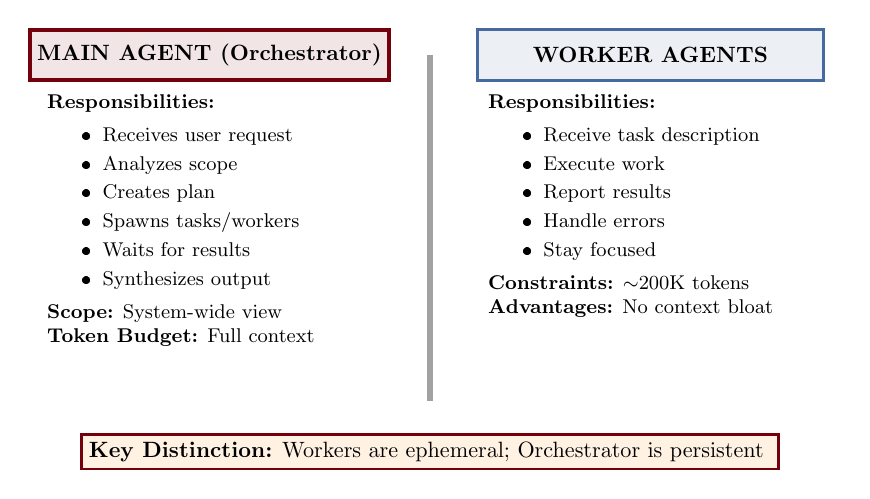
\begin{tikzpicture}[scale=0.8, transform shape]
    % Main Agent Column
    \node[orchestrator, minimum width=5.5cm, minimum height=0.8cm] (main) at (-3.5,3.5) {\textbf{MAIN AGENT (Orchestrator)}};

    \node[anchor=north west, font=\small] at (-6.2,3) {
        \begin{minipage}{5.5cm}
        \textbf{Responsibilities:}
        \begin{itemize}\setlength\itemsep{0pt}
            \item Receives user request
            \item Analyzes scope
            \item Creates plan
            \item Spawns tasks/workers
            \item Waits for results
            \item Synthesizes output
        \end{itemize}
        \textbf{Scope:} System-wide view\\
        \textbf{Token Budget:} Full context
        \end{minipage}
    };

    % Worker Agents Column
    \node[worker, minimum width=5.5cm, minimum height=0.8cm] (work) at (3.5,3.5) {\textbf{WORKER AGENTS}};

    \node[anchor=north west, font=\small] at (0.8,3) {
        \begin{minipage}{5.5cm}
        \textbf{Responsibilities:}
        \begin{itemize}\setlength\itemsep{0pt}
            \item Receive task description
            \item Execute work
            \item Report results
            \item Handle errors
            \item Stay focused
        \end{itemize}
        \textbf{Constraints:} $\sim$200K tokens\\
        \textbf{Advantages:} No context bloat
        \end{minipage}
    };

    % Divider
    \draw[line width=2pt, UofSC50Black] (0,3.5) -- (0,-2);

    % Key distinction
    \node[fill=UofSCSandstorm, draw=UofSCGarnet, line width=1pt, minimum width=10cm, align=center] at (0,-2.8) {
        \textbf{Key Distinction:} Workers are ephemeral; Orchestrator is persistent
    };
\end{tikzpicture}
\end{document}
